% IEEE QAI submission draft v5 -- adds the 2026-11-14 standard-algorithm suite (Phases A and B)
% Template: IEEEtran.cls V1.8b (IEEE conference proceedings), A4, double-blind.
% Every number in this file is checked by scripts/verify_claims.py and scripts/check_manuscript_numbers.py.
\documentclass[conference,a4paper]{IEEEtran}
\IEEEoverridecommandlockouts
\usepackage{cite}
\usepackage{amsmath,amssymb,amsthm}
\usepackage{graphicx}
\usepackage{booktabs}
\usepackage{multirow}
\usepackage[hidelinks]{hyperref}
\newtheorem{proposition}{Proposition}
\newcommand{\cmark}{yes}
\newcommand{\xmark}{no}

\begin{document}
\bstctlcite{IEEEexample:BSTcontrol}

\title{Name-Free Wire Connectivity for\\ Quantum-Circuit Learning: Exact Relabeling\\ Invariance and Width Extrapolation}

\author{\IEEEauthorblockN{Anonymous Authors}
\IEEEauthorblockA{Affiliation withheld for double-blind review}}

\maketitle

\begin{abstract}
Learned quantum-circuit models are usually trained on circuits smaller than those they must handle, and grid or sequence encodings tie each gate's position to the training size and to arbitrary qubit names. We encode a circuit as a wire-dependency directed acyclic graph (DAG) whose nodes carry only gate type, angle, and arity and whose edges record the operand roles (single-qubit, control, or target) of the two operations on their shared wire. No feature names a qubit, so per-gate predictions are exactly invariant to any permutation of logical-qubit labels. On an exactly labeled probe, predicting which gates lie on a maximum dependency path, models were trained on 4--7-qubit synthetic circuits and tested at 13--20 qubits under criteria frozen before the final runs. The DAG reaches AUROC 0.9252 against 0.8807 for a canonical-grid GRU that sees no connectivity, winning all five paired seeds. Pre-registered controls locate the source of this gain: a GRU given name-free predecessor and successor pointers on each wire ties the DAG (paired difference $-0.0023$) but loses 0.0615 AUROC when qubits are renamed. A pre-registered study on eleven standard-algorithm families compiled with Qiskit repeats both findings; there, relabeling augmentation closes the pointer GRU's gap in AUROC, though not per gate. For a label that depends on gate semantics, membership in a longest chain of the commutation-aware dependency graph, the role DAG leads the pointer GRU at 13--20 qubits in all five seeds by 0.0363, and removing operand roles costs 0.0352. Exposing connectivity without qubit names thus explains width extrapolation of a topological label; a role-labeled graph adds exact invariance everywhere and better extrapolation when the label depends on what the gates do. A held-out family and three downstream compiler tasks did not favor the DAG.
\end{abstract}

\begin{IEEEkeywords}
quantum circuits, graph neural networks, permutation invariance, out-of-distribution generalization, size generalization, critical path
\end{IEEEkeywords}

\section{Introduction}

Learning-based tools for quantum circuits face a built-in size mismatch. Labels, simulation, and compiler search are cheapest on small circuits, but the circuits of interest are larger. A learned circuit encoder therefore has to \emph{extrapolate} in width and depth, not just interpolate between familiar shapes.

Many encoders serialize a circuit as a grid or token sequence. Each gate then has a position: its layer, its token index, or its slot in a canonical order. On familiar sizes these positions correlate with structural labels, but their meaning drifts when qubits and gates are added. The same holds when logical qubits are renamed, since a canonical order must break ties using wire names. Fig.~\ref{fig:rep}(d) shows the effect on a three-qubit circuit. Swapping the names $q_0$ and $q_2$ changes the sequence positions of four of the six gates, even though the circuit is the same computation up to naming.

Other relations keep their meaning at every size and under every renaming. One example is ``this CX is the next operation, in its target role, after an RZ on the same wire.'' The wire-dependency DAG is built from exactly these relations. We encode them with \emph{operand roles} on the edges instead of absolute wire identifiers. Relabeling the qubits then leaves the input graph unchanged (Fig.~\ref{fig:rep}(c)), and the model is invariant by construction rather than by augmentation.

We ask three questions. (Q1) Can a dependency-graph encoder enforce exact invariance to logical-qubit relabeling? (Q2) Does it extrapolate better from small to much wider circuits within the same families? (Q3) If so, is the gain due to graph message passing, or to exposing which operations share a wire, and can a sequence model trained with relabeling augmentation match both properties? (Q4) Do the answers carry over to standard algorithm circuits and to a label that depends on gate semantics? Our main probe is \emph{maximum dependency-path membership}: label each gate by whether it lies on a longest path of the dependency DAG. The labels are exactly computable, so the probe has no simulator or label noise. The task isolates whether a representation supports multi-hop dependency reasoning. We do not propose the network as a replacement for the linear-time exact algorithm.

\textbf{Contributions.}
(i) An index-free circuit representation whose per-gate predictions are provably invariant to logical-qubit permutations (Proposition~\ref{prop:inv}).
(ii) A five-seed out-of-distribution benchmark with success criteria frozen before the final runs. Models train at 4--7 qubits and are tested at up to 20 qubits. The DAG beats a near-matched canonical-grid GRU without connectivity on every seed.
(iii) Pre-registered connectivity controls, whose protocols were committed before any code or result existed. A sequence model with name-free wire pointers matches the DAG's width extrapolation but not its relabeling invariance, so the gain on this probe is about \emph{exposing connectivity without names}, not about graphs as such.
(iv) A pre-registered study on eleven standard-algorithm families compiled with Qiskit. It repeats these findings for the probe label, and shows a consistent advantage of the role-labeled graph, and of operand roles, for a commutation-aware label.
(v) Supporting earlier evidence and negative results that limit the claims to within-family structural extrapolation.

\begin{figure*}[t]
\centering
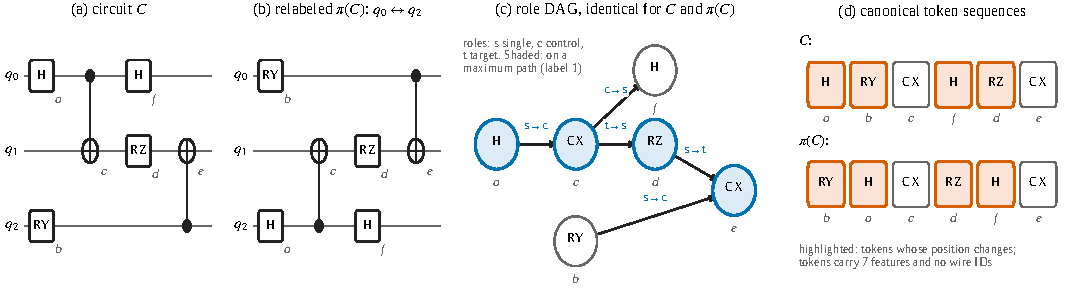
\includegraphics[width=\textwidth]{figures/fig_representation.pdf}
\caption{One circuit under two logical-qubit labelings, computed with the benchmark's own code. (a,b)~Swapping the names $q_0\leftrightarrow q_2$ is a symmetry of every structural property. (c)~The role-labeled dependency DAG, with edge attribute (source role $\rightarrow$ destination role), is identical for $C$ and $\pi(C)$, including the maximum-path labels. (d)~The canonical earliest-layer order used by the sequence baselines breaks ties with wire indices, so four of six tokens move. Italic letters mark the same operation across panels.}
\label{fig:rep}
\end{figure*}

\section{Related Work}

\emph{Circuit representations.} Graph encoders for circuits treat gates as nodes and wires as edges. QuEst predicts circuit reliability with a graph Transformer~\cite{wang2022quest}. LayerDAG generates generic DAGs layer by layer with diffusion~\cite{li2025layerdag}, and Q-Fusion adapts it to quantum circuits with learned representations of wire connections, analogous to node-type embeddings~\cite{beaudoin2025qfusion}. Any categorical vocabulary indexed by absolute wires or ordered wire pairs is defined relative to a fixed enumeration of qubits: it grows with the supported width and is not, by itself, invariant to renaming. Our encoder replaces such identities with local operand roles. This identifies a possible limitation under relabeling and width shift, not a flaw in those methods' reported results. Our implementation borrows LayerDAG-style sparse bidirectional aggregation but does not generate graphs.

\emph{Learned compilation.} Learning has been used to optimize circuits~\cite{fosel2021circuitrl} and to support routing and mapping~\cite{li2019tackling,cowtan2019qubit,preskill2018nisq}. We study a representation question that comes before such uses and make no compiler claim.

\emph{Symmetry and extrapolation.} Matching architectural symmetry to task symmetry is a central principle of geometric deep learning~\cite{bronstein2021geometric,battaglia2018relational,zaheer2017deepsets}. Message-passing networks~\cite{gilmer2017mpnn,kipf2017gcn} can learn to execute graph algorithms~\cite{velickovic2020neural}. Their extrapolation to larger graphs depends on local structure and on how well the architecture is aligned with the algorithm~\cite{yehudai2021size,xu2021extrapolate}. Our longest-path probe sits in this algorithmic-alignment setting.

\section{Representation and Invariance}

\subsection{Wire-dependency DAG with operand roles}
A circuit $C=(o_1,\dots,o_m)$ on logical qubits $Q$ is an ordered list of operations $o_i=(g_i,\mathbf{w}_i,\theta_i)$. Here $g_i\in\{\mathrm{H},\mathrm{RY},\mathrm{RZ},\mathrm{CX}\}$, $\mathbf{w}_i$ is a tuple of distinct qubits (control first for CX), and $\theta_i$ is an angle (0 if absent). For each $q\in Q$, let $i_1<\dots<i_k$ index the operations that act on $q$. We add a directed edge $(i_j\to i_{j+1})$ for each consecutive pair. The union over all wires is the dependency DAG $G(C)$; independent operations are never connected. The role of qubit $q$ in operation $i$ is $r(i,q)\in\{\mathrm{s},\mathrm{c},\mathrm{t}\}$ (single-qubit operand, CX control, or CX target). The edge $(i_j\to i_{j+1})$ induced by $q$ carries the six-dimensional attribute $[\mathrm{onehot}(r(i_j,q)),\mathrm{onehot}(r(i_{j+1},q))]$. Each node carries seven features: a four-way gate one-hot, $\sin\theta_i$, $\cos\theta_i$, and arity$/2$. No feature names a wire.

The network has six residual blocks. Each block applies separate linear messages to (sender state $\Vert$ edge roles) along forward and backward edges, sums them with \texttt{index\_add}, and applies a self transform, a GELU, and LayerNorm. A linear head outputs one logit per gate. The model has 80,833 parameters.

\subsection{Exact invariance}
\begin{proposition}\label{prop:inv}
Let $\pi$ be any permutation of $Q$ and $\pi(C)=(g_i,\pi(\mathbf{w}_i),\theta_i)_{i=1}^m$. Then $G(\pi(C))$ and $G(C)$ have identical node features and identical multisets of attributed edges. Consequently, any model that consumes the node features and an unordered multiset of attributed edges receives identical input for $C$ and $\pi(C)$, and so satisfies $f(\pi(C))_i=f(C)_i$ for every $i$. The sum-aggregation network above is such a model. The labels satisfy $y(\pi(C))=y(C)$.
\end{proposition}
\begin{proof}
Node features do not depend on $\mathbf{w}_i$. Operation $i$ acts on $\pi(q)$ in $\pi(C)$ exactly when it acts on $q$ in $C$, so the ordered chain of operations on wire $\pi(q)$ equals the chain on $q$. Because $\pi$ is applied entrywise, $q$'s position in $\mathbf{w}_i$ equals $\pi(q)$'s position in $\pi(\mathbf{w}_i)$, so $r(i,\pi(q))=r(i,q)$. The edges contributed by wire $\pi(q)$ in $\pi(C)$ are therefore exactly those contributed by $q$ in $C$, with the same endpoints and attributes. Because no attribute records the wire, the two edge multisets coincide. Sum aggregation does not depend on edge order, so every layer, and hence every logit, agrees. The labels depend only on the edge structure.
\end{proof}
Because the model is permutation-equivariant over nodes, its predictions also follow any legal reordering of commuting operations. The guarantee is exact in exact arithmetic; the protocol tolerance of $10^{-6}$ allows for floating-point summation order.

\subsection{Sequence baselines and what each model receives}
Both baselines receive the same seven index-free node features. Gates are sorted by the key (earliest dependency layer, wire tuple, gate, angle). The \emph{canonical-grid GRU}~\cite{cho2014gru} (two bidirectional layers, width 96, 84,961 parameters) reads this sequence. The \emph{canonical Transformer}~\cite{vaswani2017attention} (width 64, two layers, four heads, feed-forward width 160, learned positions for up to 192 tokens, no dropout, 88,065 parameters) reads the same sequence. Table~\ref{tab:access} states what each model sees. The sequence models get no wire identifiers and no explicit connectivity: shared-wire structure reaches them only through the canonical order, and wire names enter that order only as a tie-breaker. The primary comparison is therefore between an index-free encoding that \emph{exposes} dependency relations and index-free serializations that \emph{do not}.

\emph{Connectivity controls.} To separate connectivity from graph structure, a \emph{pointer GRU} (87,457 parameters) reads the same canonical sequence with 26 extra features per token. For each operand (control or single-qubit operand first, then target) it receives the operand's role and, for the previous and the next operation on the same wire, an existence flag, that operation's role, and the log canonical-position distance. Wire names are used only to find these neighbors and are never emitted. Roles and existence flags are invariant to relabeling, but the distances are measured in the canonical order, whose tie-breaks depend on names, so the model is not invariant. A \emph{pointer Transformer} (89,729 parameters) uses the same features with the Transformer configuration above. A \emph{role-ablated DAG} sets every edge attribute to zero, keeping topology only.

\begin{table}[t]
\centering
\caption{Inputs and properties of the compared encoders}
\label{tab:access}
\setlength{\tabcolsep}{2pt}
\begin{tabular}{@{}lcccc@{}}
\toprule
 & Role DAG & Grid GRU & Transf. & Ptr.\ GRU \\
\midrule
Gate, $\sin\theta$, $\cos\theta$, arity & \cmark & \cmark & \cmark & \cmark \\
Shared-wire connectivity & edges & implicit & implicit & pointers \\
Operand roles & on edges & \xmark & \xmark & per token \\
Order depends on names & \xmark & tie-breaks & tie-breaks & tie-breaks \\
Exactly invariant & \cmark & \xmark & \xmark & \xmark \\
Parameters & 80,833 & 84,961 & 88,065 & 87,457 \\
Evidence tier & primary & primary & post & post \\
\bottomrule
\end{tabular}
\end{table}

\subsection{Probe task}
Let $a(v)$ be the number of operations on the longest dependency path ending at $v$, $b(v)$ the number on the longest path starting at $v$, and $D=\max_v a(v)$. The label is $y_v=\mathbf{1}[a(v)+b(v)-1=D]$, meaning $v$ lies on at least one maximum path. It is computed exactly in linear time. Positive rates are 0.700, 0.568, and 0.517 on the same-size, near-width, and far-width test sets.

\section{Experimental Protocol}

\emph{Data.} Circuits come from three seeded generators with equal shares. QAOA-like circuits consist of a Hadamard layer followed by alternating CX--RZ--CX cost blocks and H--RZ--H mixer blocks~\cite{farhi2014qaoa}. Hardware-efficient VQE circuits~\cite{peruzzo2014vqe} use RY/RZ layers and cyclically offset CX entanglers. Reversible linear arithmetic uses pivot-controlled CX fans with RZ phases. Training uses 1,000 circuits with 4--7 qubits and 32--64 gates; validation uses 256 fresh circuits. Each of four final splits has 512 circuits: \emph{same size} (4--7 qubits, 32--64 gates), \emph{near width} (8--12, 72--104), \emph{far width} (13--20, 96--144), and \emph{relabeled} (the same-size circuits after an independent random qubit permutation per circuit). Content hashes of all splits are stored with the results, regenerating the splits reproduces them, and no test circuit duplicates a training circuit.

\emph{Training.} Each model trains for 4,000 AdamW updates (learning rate $3\times10^{-4}$, batch 16, clipping 1.0, positive-class weighting) under paired seeds 111--115. A given seed fixes the initialization stream and the minibatch indices for both architectures. The checkpoint is chosen by validation AUROC, evaluated every 250 updates. The final splits are never used for training or selection.

\emph{Frozen gate.} A development run on separate data (one seed, 2,000 updates) fixed the architectures and size ranges. According to the project records (see the provenance note in Section~\ref{sec:limits}), the final protocol then fixed these success criteria before the final data were generated. (1) The DAG's far-width AUROC exceeds the grid's in all five seeds. (2) The mean improvement is at least $+0.03$. (3) The DAG's mean far-width F1 exceeds the grid's. (4) The maximum change in DAG logits under relabeling is at most $10^{-6}$. (5) The DAG's same-size metrics are unchanged by relabeling.

\emph{Evidence tiers.} \emph{Primary confirmatory:} the five-seed DAG-versus-grid final. \emph{Post-confirmatory controls:} the Transformer, whose configuration was fixed after the primary result had been opened, and the connectivity controls, augmentation control, and standard-algorithm suite, whose protocols, including pass/fail readings, were committed and pushed to the project repository before their code was written. None received any tuning. \emph{Supporting:} two earlier frozen studies with a different, wire-indexed architecture (Section~\ref{sec:limits}). We never pool statistics across tiers.

\emph{Statistics.} We report node-level AUROC and F1 (threshold 0.5), with means and sample standard deviations over the five training seeds. Each seed's DAG and grid share data and minibatches, so we report per-seed paired differences and a descriptive Student-$t$ interval over seeds ($\mathrm{df}=4$). The test sets are fixed, so this interval covers training randomness only, not sampling of circuits. Gates within a circuit are not independent, and we do not treat them as replicates.

\emph{Standard-algorithm suite.} A final pre-registered study replaces the synthetic generators with eleven families built from Qiskit's circuit library~\cite{qiskit2024} with randomized instances: QFT on random product states, phase estimation, Bernstein--Vazirani and Deutsch--Jozsa oracles, graph states, MaxCut QAOA, hardware-efficient and excitation-preserving ans\"atze, Trotterized Heisenberg and Ising evolution, ripple-carry adders, quantum-volume layers, and IQP circuits. The Qiskit transpiler (optimization level 1, no coupling map) compiles each circuit to the same four-gate basis, so the encoders are unchanged. Training uses 1,100 circuits with 4--7 qubits and validation 264. The same-size, near-width, and far-width test splits have 528 circuits each, with up to 1,191 gates at far width, and no circuit repeats within or across splits. Two renamings are evaluated: a random permutation, and reversal of the qubit order, the endianness convention that differs between frameworks. \emph{Phase A} keeps the probe label. \emph{Phase B} labels membership in a longest chain of the commutation-aware dependency DAG computed by Qiskit, which depends on gate semantics: an RZ commutes with a CX on its control but not on its target. The two labels disagree on 28\% of training gates and 36\% of far-width gates. Family sizes differ by a factor of 33 at far width, so the primary metric is the \emph{family-macro} AUROC, the mean of within-family node AUROCs. The oracle family is all-positive under the Phase B label and is left out there. The role DAG, grid GRU, pointer GRU, augmented pointer GRU and, in Phase B, the role-ablated DAG were trained with the unchanged recipe and seeds; the Transformers cannot read circuits beyond their 192 positions. The protocol, with a reading for each conclusion, was pushed before the run code existed, and the data manifest before training.

\section{Results}

\begin{table}[t]
\centering
\caption{Frozen five-seed final: AUROC (mean $\pm$ s.d.) and F1}
\label{tab:main}
\setlength{\tabcolsep}{2.4pt}
\resizebox{\columnwidth}{!}{%
\begin{tabular}{@{}lccccc@{}}
\toprule
 & \multicolumn{2}{c}{Role DAG (primary)} & \multicolumn{2}{c}{Grid GRU (primary)} & Transf.$^\dagger$ \\
\cmidrule(lr){2-3}\cmidrule(lr){4-5}\cmidrule(l){6-6}
Split & AUROC & F1 & AUROC & F1 & AUROC \\
\midrule
Same, 4--7 q & $.9722{\pm}.0009$ & .9383 & $.9391{\pm}.0028$ & .8919 & $.8888{\pm}.0010$ \\
Near, 8--12 q & $.9362{\pm}.0008$ & .8749 & $.8853{\pm}.0027$ & .8034 & $.7467{\pm}.0070$ \\
Far, 13--20 q & $.9252{\pm}.0020$ & .8458 & $.8807{\pm}.0045$ & .8011 & $.7471{\pm}.0128$ \\
Relabeled & $.9722{\pm}.0009$ & .9383 & $.8294{\pm}.0053$ & .8199 & $.7806{\pm}.0064$ \\
\bottomrule
\end{tabular}}\\[2pt]
\footnotesize{$^\dagger$Post-confirmatory descriptive control, not part of the frozen gate. Its F1 (same/near/far/relabeled) is .8543/.7427/.7263/.8064.}
\end{table}

\begin{figure}[t]
\centering
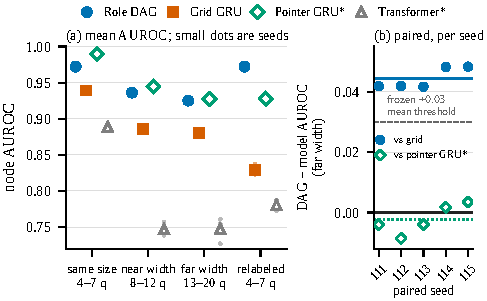
\includegraphics[width=\columnwidth]{figures/fig_results.pdf}
\caption{(a)~Mean AUROC per split, with individual seeds as small dots. Open markers (*) are post-confirmatory controls. (b)~Paired far-width differences, DAG minus model. Against the grid (filled) all five seeds clear zero and the mean clears the frozen $+0.03$ threshold; against the pointer GRU (open) the differences straddle zero.}
\label{fig:results}
\end{figure}

\subsection{Primary result: width extrapolation}
All five gate conditions pass (Table~\ref{tab:main}, Fig.~\ref{fig:results}). The paired far-width AUROC differences (DAG minus grid) are positive in all five seeds, with mean $+0.0444$ (s.d.\ 0.0035) and a descriptive seed-level 95\% $t$ interval of $[+0.0400,+0.0488]$. The DAG's far-width F1 is 0.8458 against 0.8011. The DAG also leads at the same size ($+0.0331$ AUROC) and at near width ($+0.0509$), so the advantage is not specific to extrapolation, but it holds up to 20 qubits, roughly three times the training width.

\subsection{Logical-qubit relabeling}
On the 64 circuit--relabeling pairs checked per seed, the largest change in any DAG logit is exactly 0.0, and the DAG's metrics are identical on the original and relabeled splits. A post-hoc re-run of seed 111 reproduced every recorded AUROC bit for bit, with a maximum DAG logit change of 0.0 over all 512 relabeled circuits. The grid's AUROC drops from 0.9391 to 0.8294 ($-0.1097$) and the Transformer's from 0.8888 to 0.7806. Removing explicit wire indices from a serialization therefore does not make it invariant; the computation itself has to respect the symmetry. Section~\ref{sec:controls} tests relabeling augmentation.

\emph{Transformer control.} The canonical Transformer, added after the primary result was known and not tuned, is weaker than both primary models on every split (far width 0.7471). The conclusion therefore does not hinge on a recurrent baseline, although a tuned attention model could do better.

\subsection{Post-confirmatory connectivity controls}\label{sec:controls}
\begin{table}[t]
\centering
\caption{Connectivity and augmentation controls (post-confirmatory): AUROC (mean $\pm$ s.d.) and DAG$-$model far-width paired differences}
\label{tab:controls}
\setlength{\tabcolsep}{2.4pt}
\resizebox{\columnwidth}{!}{%
\begin{tabular}{@{}lccccc@{}}
\toprule
 & Role & Pointer & Ptr.\ GRU & Pointer & Role-abl. \\
Split & DAG & GRU & + aug. & Transf. & DAG \\
\midrule
Same, 4--7 q & $.9722{\pm}.0009$ & $.9895{\pm}.0010$ & $.9757{\pm}.0018$ & $.9481{\pm}.0019$ & $.9670{\pm}.0013$ \\
Near, 8--12 q & $.9362{\pm}.0008$ & $.9447{\pm}.0026$ & $.9296{\pm}.0012$ & $.7533{\pm}.0168$ & $.9282{\pm}.0019$ \\
Far, 13--20 q & $.9252{\pm}.0020$ & $.9274{\pm}.0050$ & $.9149{\pm}.0027$ & $.6900{\pm}.0192$ & $.9199{\pm}.0025$ \\
Relabeled & $.9722{\pm}.0009$ & $.9279{\pm}.0044$ & $.9721{\pm}.0017$ & $.8838{\pm}.0035$ & $.9670{\pm}.0013$ \\
Far, relabeled & $.9252$ (exact) & --- & $.9173{\pm}.0029$ & --- & exact \\
Max $|\Delta|$ logit & 0.0 & 19.2 & 10.8 & 27.2 & 0.0 \\
\midrule
DAG$-$model, far & --- & $-.0023$ & $+.0103$ & $+.2352$ & $+.0053$ \\
DAG wins (of 5) & --- & 2 & 5 & 5 & 5 \\
\bottomrule
\end{tabular}}\\[2pt]
\footnotesize{Role DAG values are the recorded primary results; its far-relabeled value follows from Proposition~\ref{prop:inv}. Max $|\Delta|$ logit is over 64 same-size circuit--relabeling pairs per seed. A re-run of seed 112 in the controls' software environment reproduced every recorded DAG and grid AUROC bit for bit.}
\end{table}

Table~\ref{tab:controls} answers Q3. Before any code existed, the protocol fixed the reading \emph{information explains the gap} if the DAG's mean far-width lead over the pointer GRU is below $+0.01$ or the pointer GRU wins at least three seeds, and \emph{topology supported} if the DAG wins all five seeds by at least $+0.02$ on average. The pointer GRU wins three seeds and the paired difference is $-0.0023$ (s.d.\ 0.0049, interval $[-0.0083,+0.0038]$): \emph{information explains the gap}. Given name-free wire pointers, a plain bidirectional GRU matches the DAG at 13--20 qubits, beats it at the training size (0.9895), and exceeds the canonical grid by $+0.0467$ at far width. At the 0.5 threshold the DAG keeps a higher far-width F1 (0.8458 against 0.8081, all five seeds), a difference in calibration under shift that was not a pre-declared criterion. The pointer GRU is not invariant: its AUROC falls by 0.0615 under relabeling, to 0.9279.

The pointer Transformer collapses with width (0.6900), probably because its learned absolute positions never see sequences this long. Removing operand roles from the DAG lowers far-width AUROC by 0.0053 (interval $[+0.0019,+0.0086]$, all five seeds), below the protocol's 0.01 threshold: roles are \emph{not needed} for this probe.

\emph{Relabeling augmentation.} A second protocol, also pushed before its code, retrained the pointer GRU with every sampled training circuit freshly relabeled (same minibatch indices, no tuning). Its readings are \emph{suffices} if both relabeling AUROC gaps are at most 0.005 and the DAG's far-width lead is at most 0.01, and \emph{insufficient} if a gap or the lead is at least 0.02. The augmented model's gaps are 0.0035 at 4--7 qubits and $-0.0024$ on a relabeled copy of the far-width split, so near-invariance learned at training size carries to larger widths. Its far-width AUROC falls to 0.9149, and the DAG leads in all five seeds by $+0.0103$ (interval $[+0.0055,+0.0150]$): \emph{intermediate}. Renaming still moves its predicted probabilities by 0.053 on average, against exactly zero for the DAG. Augmenting the canonical grid removed its relabeling gap but lowered its far-width AUROC to 0.8657, so tie-break order had been carrying information.

\subsection{Standard-algorithm circuits}\label{sec:suite}
\begin{table}[t]
\centering
\caption{Standard-algorithm suite (post-confirmatory): family-macro AUROC (mean $\pm$ s.d.) and DAG$-$model far-width paired differences}
\label{tab:suite}
\setlength{\tabcolsep}{2.4pt}
\resizebox{\columnwidth}{!}{%
\begin{tabular}{@{}lccccc@{}}
\toprule
 & Role & Pointer & Ptr.\ GRU & Grid & Role-abl. \\
Split & DAG & GRU & + aug. & GRU & DAG \\
\midrule
\multicolumn{6}{@{}l}{\emph{Phase A: wire-dependency path label (the probe)}} \\
Same, 4--7 q & $.9803{\pm}.0012$ & $.9920{\pm}.0004$ & $.9884{\pm}.0004$ & $.9663{\pm}.0009$ & --- \\
Far, 13--20 q & $.9455{\pm}.0010$ & $.9442{\pm}.0040$ & $.9450{\pm}.0044$ & $.8617{\pm}.0231$ & --- \\
Far, relabeled & $.9455$ (exact) & $.9205{\pm}.0056$ & $.9463{\pm}.0039$ & $.7961{\pm}.0234$ & --- \\
DAG$-$model, far & --- & $+.0013$ & $+.0005$ & $+.0838$ & --- \\
DAG wins (of 5) & --- & 3 & 4 & 5 & --- \\
\midrule
\multicolumn{6}{@{}l}{\emph{Phase B: commutation-aware chain label}} \\
Same, 4--7 q & $.9635{\pm}.0016$ & $.9562{\pm}.0017$ & $.9476{\pm}.0017$ & $.9222{\pm}.0009$ & $.9376{\pm}.0013$ \\
Far, 13--20 q & $.9354{\pm}.0006$ & $.8991{\pm}.0046$ & $.8933{\pm}.0055$ & $.8243{\pm}.0105$ & $.9002{\pm}.0026$ \\
Far, relabeled & $.9354$ (exact) & $.8516{\pm}.0030$ & $.8921{\pm}.0039$ & $.7505{\pm}.0079$ & exact \\
DAG$-$model, far & --- & $+.0363$ & $+.0421$ & $+.1111$ & $+.0352$ \\
DAG wins (of 5) & --- & 5 & 5 & 5 & 5 \\
\bottomrule
\end{tabular}}
\end{table}

\emph{Phase A (probe label).} Every reading matches or strengthens the synthetic study (Table~\ref{tab:suite}). Both connectivity models beat the grid GRU at far width in every seed (DAG $+0.0838$, pointer GRU $+0.0825$; reading \emph{replicated}), and the DAG and the pointer GRU \emph{tie} ($+0.0013$, interval $[-0.0033,+0.0060]$). Renaming costs the unaugmented pointer GRU 0.0237 at far width under a random permutation and 0.0362 under order reversal; the grid loses 0.0656 and 0.0828. With augmentation the pointer GRU's gaps close (0.0005 at 4--7 qubits, $-0.0013$ at far width) and the DAG's lead is $+0.0005$, so the reading here is \emph{suffices}, where the synthetic families gave \emph{intermediate}. Invariance per gate is still not reached: renaming moves the augmented model's far-width probabilities by 0.072 on average, against exactly zero for the DAG on all 2,112 renamed circuits per seed. The macro tie hides opposite family effects: the pointer models are better on the random-graph families (graph states, IQP, QAOA), and the DAG on QFT, phase-estimation, quantum-volume, and hardware-efficient circuits. At the 0.5 threshold the DAG's far-width F1 is 0.9738, against 0.8112 and 0.9004 for the pointer models.

\emph{Phase B (commutation-aware label).} Here the graph has an advantage. The DAG leads the pointer GRU in all five seeds by $+0.0363$ (interval $[+0.0303,+0.0422]$; reading \emph{graph advantage}) and the augmented pointer GRU by $+0.0421$ ($[+0.0351,+0.0491]$). Augmentation again removes the relabeling gap in AUROC (at most 0.0012) but not the accuracy deficit, so its reading is \emph{insufficient} by the lead criterion. Removing operand roles costs the DAG 0.0352 in every seed ($[+0.0323,+0.0381]$; reading \emph{roles contribute}), against 0.0053 on the synthetic probe: whether a neighbor acts as control or target decides whether two gates commute. The DAG also leads at the training size (0.9635 against 0.9562), and its margin grows with width. Connectivity still helps the sequence model (pointer GRU $+0.0748$ over the grid; \emph{replicated}).

\section{Limitations and Negative Results}\label{sec:limits}

\emph{Scope of the labels.} Both labels are computed exactly by classical algorithms, in linear time for the probe and in polynomial time for the commutation-aware chain. They test representational inductive bias, not usefulness; a compiler should compute them directly. The primary study uses synthetic generators. The suite uses library constructions of standard algorithms under one compilation setting, not circuits from deployed applications. All circuits use four gate types and are noise-free, and nothing is executed on hardware.

\emph{Earlier studies and unseen families.} Two earlier frozen studies used a different architecture in which both models received absolute wire one-hots (at most 12 wires); they are not pooled with the results above. On the three synthetic families, adding wires gave the DAG $+0.0514$ AUROC over the grid and adding depth alone $+0.0025$, which motivated removing wire identifiers. On random circuits the grid was better at the training size (0.9406 against 0.8556) but worse on larger circuits (0.7861 against 0.8078). On a held-out chemistry-inspired family both models were near chance and the grid led by $0.0266$. Every family in the suite was seen in training, so family transfer remains unshown.

\emph{Downstream tasks.} Three compiler-facing follow-ups did not establish a DAG advantage. In small-angle deletion ranking, a simple heuristic saturated the task. In safe identity-rewrite prioritization, the DAG was favored in all three final seeds, but its $+0.0379$ oracle-recovery gain missed the frozen $+0.05$ threshold. In routed-rewrite selection, the development runs favored the grid (6.30 against 6.66 routed CX gates removed on average), and no final test was opened. In a separate state-preparation study, a DAG generator reached fidelity 0.99 on only 9 of 128 targets. We claim no compiler or generation advantage.

\emph{What the DAG does and does not provide.} For the probe label, width extrapolation is matched by a sequence model with name-free wire pointers, and on standard-algorithm circuits augmentation also closes the accuracy gap. The primary gain over the canonical grid should therefore not be attributed to graph message passing; the DAG's distinct benefit there is exact per-gate invariance. Its accuracy advantage appears for one commutation-aware label on one suite, with untuned models on both sides; a tuned or relative-position sequence model might narrow it.

\emph{Statistical and design limits.} Five seeds on fixed test sets bound training variance only. No model was tuned; relative-position attention and symmetry-aware graph Transformers remain untested. The models are near-matched (80,833 to 89,729 parameters), not exactly matched.

\emph{Provenance.} The protocols, code, and results are archived with dataset hashes, per-seed training histories, and a compute ledger (CPU only). According to the project records, each primary and supporting protocol was written before its final run, but those protocols were committed together with their results, so the repository alone does not timestamp them independently. The control and suite protocols were committed and pushed before their code and results; the connectivity protocol records one correction (its text called every pointer feature relabeling-invariant, which is false for the distance features). The implementation follows LayerDAG's design in native PyTorch, without runtime parity with the upstream code.

\section{Conclusion}
Operand-role dependency graphs encode the symmetry of logical-qubit relabeling by construction. In a frozen experiment on synthetic families, the role DAG beat a near-matched canonical-grid GRU at 13--20 qubits on all five paired seeds (AUROC 0.9252 against 0.8807) after training at 4--7 qubits. Pre-registered controls show where that gain comes from: a GRU given name-free predecessor and successor pointers matches the DAG at width, on the synthetic families and on eleven standard-algorithm families alike. Exposing wire connectivity without qubit names is what drives width extrapolation of a topological label. The dependency graph is the only encoder tested that is exactly invariant: the pointer GRU loses accuracy when qubits are renamed or their order is reversed, and relabeling augmentation restores its AUROC but not its per-gate predictions. When the label depends on gate semantics, as in commutation-aware chains, the role-labeled graph extrapolates better than either pointer model in every seed, and its operand roles matter. The results do not establish robustness to unseen families or a practical compiler advantage.

\section*{Acknowledgment}
Funding and acknowledgments are withheld for double-blind review. In accordance with IEEE policy on AI-generated content, the authors disclose that a large language model (Anthropic Claude) was used to edit and restructure the manuscript text, to generate figure-plotting code, to implement and run the post-confirmatory controls and the standard-algorithm suite under author-approved protocols, and to audit the manuscript's numbers against the machine-readable results. The authors take responsibility for all content.

\bibliographystyle{IEEEtran}
\bibliography{references}

\end{document}
